\documentclass[brazil,12pt,a4paper,openany]{article}
\usepackage{anysize}
\usepackage[utf8]{inputenc}
\usepackage[portuguese]{babel}
\usepackage[ruled]{algorithm}
\usepackage{makeidx}
%\usepackage{abntex2} 
%%%%%%%%%%%%%%%%%%%%%%%%%%%%%%%%%%
%\usepackage{color,footnote}
\usepackage{babel}
%\usepackage{amsmath,amssymb}
\usepackage{mathtools,bbm}
\usepackage{subfigure}
%\usepackage{subfig}
%\usepackage{graphicx}
\usepackage{svg}%include figure svg
\usepackage{physics,braket}
\usepackage{comment}
\usepackage{caption}
\usepackage{subcaption}
%\usepackage{mathtools,mathrsfs}
\usepackage[normalem]{ulem}
\usepackage[varg]{txfonts} 
\usepackage{mathtools,mathrsfs}
\usepackage{amsmath,amssymb}
%%%%%%%%%%%%%%%%%%%%%%%%%%%%%%%%%%
%\usepackage{subfig}

\usepackage{amsmath}
\usepackage{amssymb}
% \usepackage{amsthm}
\usepackage{mathrsfs}
\usepackage{graphicx}
\usepackage{fancyhdr}
\usepackage{array}
\usepackage{geometry}
\usepackage{simplewick}
\usepackage{latexsym}
\usepackage[all]{xy}
%\usepackage{eufrak}
\usepackage{euscript}
\usepackage{enumerate}
\usepackage{dsfont}
\usepackage{slashed}
\usepackage{hyperref}
\usepackage[nottoc]{tocbibind}
\usepackage{lscape}
\graphicspath{ {images/} }
\usepackage{setspace}
%\usepackage[usenames, dvipsnames]{xcolor}
\usepackage{xcolor}
\setstretch{0.93}
\makeindex

\usepackage{etoolbox}
\makeatletter
\patchcmd{\chapter}{\if@openright\cleardoublepage\else\clearpage\fi}{}{}{}
\makeatother

\marginsize{20mm}{20mm}{20mm}{20mm}

\hypersetup{colorlinks=true,breaklinks=true,linkcolor=black,citecolor=black,
urlcolor=black}


\def\s{\sigma}
\def\ave#1{\langle #1\rangle}
%\newcommand{\bra}[1]{\langle #1|}
%\newcommand{\ket}[1]{|#1\rangle}
%\newcommand{\braket}[2]{\langle #1|#2\rangle}
\newcommand{\iv}{\mathbf{i}}
\newcommand{\jv}{\mathbf{j}}
\newcommand{\kv}{\mathbf{k}}
\newcommand{\dbar}{{\mathchar'26\mkern-11mud}}
\newcommand{\mf}{\mathfrak}

\newcommand*{\img}[1]{%
    \raisebox{-.2\baselineskip}{%
        \includegraphics[
        height=\baselineskip,
        width=\baselineskip,
        keepaspectratio,
        ]{#1}%
    }%
}
\begin{document}

\setlength{\abovecaptionskip}{0.0cm}
\setlength{\belowcaptionskip}{0.0cm}
%\setlength{\baselineskip}{24pt}

\pagestyle{fancy}
\lhead{}
\chead{}
\rhead{\thepage}
\lfoot{}
\cfoot{}
\rfoot{}

\fancypagestyle{plain}
{
	\fancyhf{}
	\lhead{}
	\chead{}
	\rhead{\thepage}
	\lfoot{}
	\cfoot{}
	\rfoot{}
}

\renewcommand{\headrulewidth}{0pt}



%%%%%%%%%%%%%%%%%%%%%%%%%%%%%%%%% Capa %%%%%%%%%%%%%%%%%%%%%%%%%%%%%%%%%%


%\mainmatter

\begin{center}

{\Large \bf Projeto de doutorado-sanduíche  CAPES-PDSE - EDITAL Nº 09/2024 

Fonte de single fótons via espalhamento Raman }

\vspace{15pt}

{\large  Thiago Elbert Guimarães}

\end{center}
%\vspace{270pt}
\begin{center}
19 de Novembro de 2024
\end{center}
%\newpage


\section{Introdução}
\label{intro2}
A mecânica quântica transformou nossa compreensão da natureza ao introduzir conceitos revolucionários, como superposição e emaranhamento, que contrastam fortemente com a intuição clássica \cite{feynman1965feynman,bell1964einstein}. Esses princípios não apenas desafiam as concepções convencionais, mas também estabelecem as bases para uma nova era de inovação tecnológica \cite{dowling2003quantum}. O estudo de sistemas quânticos é essencial para aprofundarmos nossa compreensão e habilidade de manipular esses fenômenos.

Entre os métodos que exploram esses fenômenos, a Conversão Paramétrica Descendente Espontânea (SPDC) se destaca como uma técnica eficaz para a geração de luz emaranhada. Nesse processo, um fóton de energia \(\omega_L\) é convertido em dois fótons de energias \(\omega_s\) e \(\omega_i\), obedecendo às leis de conservação de energia (\(\omega_L = \omega_i + \omega_s\)) e de momento (\(k_L = k_s + k_i\)). Esse processo não linear de segunda ordem permite a criação de pares de fótons emaranhados, amplamente utilizados em experimentos de teste de desigualdades de Bell \cite{weihs1998violation}, criptografia quântica \cite{jennewein2000quantum} e teleporte quântico \cite{bouwmeester1997experimental}.

Além da SPDC,  outras fontes de fótons emaranhados foram desenvolvidas com o objetivo de optimizar a eficiência de produção e a pureza do estado emaranhado. Entre elas estão os Pontos Quânticos \cite{Stevenson2006Dots} e os sistemas de espalhamento Raman \cite{Jorio2017Cooper}. No espalhamento Raman, um fóton é absorvido e gera outro fóton com uma energia diferente devido ao espalhamento inelástico com a matéria. No processo Stokes (S), um fóton com desvio para o vermelho é gerado quando parte de sua energia é transferida para um quantum de vibração atômica (fônon, em sólidos). Já o processo anti-Stokes (aS), que resulta em um deslocamento para o azul, é menos comum, pois requer uma excitação vibracional pré-existente. O espalhamento aS entre um fóton incidente e um fônon criado no cristal pelo espalhamento S prévio é o chamado processo Stokes-anti-Sokes (SaS) e gera pares de fótons correlacionados.

Nesses processos, os pares de fótons são gerados através de interações mediadas por fônons, destacando a correlação temporal entre eles e suas implicações para aplicações em informação quântica \cite{de2019physical}. Estudos recentes investigaram as propriedades desses fótons correlacionados, explorando como as interações fotônicas são mediadas por fônons virtuais e analisando a produção de pares Stokes–anti-Stokes em função da energia, momento e outras características físicas, sugerindo analogias com a teoria BCS da supercondutividade \cite{junior2019stokes}. Além disso, foram investigadas as correlações temporais e a polarização dos pares de fótons Stokes–anti-Stokes em processos reais e virtuais de espalhamento Raman em diamante, revelando diferenças fundamentais entre os processos reais (limitados pela vida útil dos fônons) e os virtuais (limitados pela largura de pulso do laser de excitação) \cite{junior2020lifetime}.

Outro aspecto interessante do SaS correlacionado está relacionado à conservação de momento, que pode ser investigado analisando-se a correlação espacial transversal dos pares. Em geral, os fótons espalham-se em várias direções ao interagir com fônons, resultando em um perfil de intensidade Raman que se desvia da direção de propagação do feixe de laser incidente. No entanto, o SaS correlacionado preserva o mesmo perfil espacial definido pelo laser de excitação, seguindo o caminho do feixe incidente, o que se assemelha ao comportamento observado na transferência de perfil de amplitude na SPDC \cite{junior2019stokes}.

%Neste projeto, buscamos explorar o processo SaS investigando os modos transversais da luz, como o modo Laguerre-Gaussiano, que pode carregar momento angular orbital.

Na próxima seção, apresentamos as justificativas do projeto, destacando sua contribuição para a formação de recursos humanos de alto nível para inserção nos meios acadêmico, de ensino e de pesquisa no país. Em seguida, delineamos nossos Objetivos e Metodologia nas Seções 3 e 4, respectivamente, enquanto os Resultados Esperados e Impacto do Projeto são discutidos na Seção 5, enfatizando sua relevância para o desenvolvimento científico da área em médio e longo prazo. Por fim, o Cronograma é apresentado na Seção 6.

\section{Justificativa}

Este projeto integra as atividades do Laboratório de Óptica e Informação Quântica (LOIQ), do Instituto de Física da UFRJ, em colaboração com o IDOR, e busca contribuir para o desenvolvimento de fontes de fótons mais eficientes para aplicações em informação quântica, comunicação e sensoriamento. A geração controlada de fótons individuais e de pares correlacionados é uma etapa essencial para a implementação de tecnologias quânticas, pois influencia diretamente a eficiência, a estabilidade e a escalabilidade dos experimentos.

Embora fontes baseadas em Conversão Paramétrica Descendente Espontânea (SPDC) sejam amplamente utilizadas, processos de espalhamento Raman Stokes--anti-Stokes oferecem uma alternativa promissora, especialmente em sistemas de estado sólido como o diamante. Nesse contexto, o uso de guias de onda escritas por laser de femtossegundo pode aumentar o confinamento da luz e favorecer o acoplamento fóton-fônon, ampliando a eficiência de geração de pares correlacionados.

Além de seu interesse científico fundamental, o projeto contribui para a formação de recursos humanos em óptica quântica experimental, espectroscopia Raman e fotônica integrada. Seus resultados poderão fortalecer o desenvolvimento de fontes compactas e integráveis de luz quântica, com impacto potencial em comunicação, sensoriamento e processamento de informação baseados em princípios quânticos.

%%%%%%%%%%%%%%%%%%%%%%%%%%%%%%%%%%%%%%%%%%%%%%%%%%%%%%%%%%%%%%%%%%%%%


\section{Objetivo e Metodologia}

%\section{Metodologia}
Na espectroscopia Raman, um laser com frequência $\omega_L$ incide sobre um material, que gera luz em diferentes frequências por meio de dispersão inelástica fraca. A contribuição mais abundante nesse tipo de espalhamento é o processo de Stokes (S), que ocorre quando um fóton do laser é absorvido pelo material, criando uma vibração quântica com frequência $\nu$ (vibração para líquidos, fônon para sólidos) e um fóton de menor energia $\omega_S$, conhecido como fóton Stokes, conforme ilustrado no diagrama de Feynman na Figura \ref{S-aS} a). Além disso, o efeito Raman permite a criação de fótons com maior energia no processo anti-Stokes (aS), mostrado na Figura \ref{S-aS} b). Esse processo ocorre quando o material transfere a energia $\nu$ de uma molécula previamente excitada para o fóton do laser incidente de energia $\omega_L$, criando um fóton com maior energia $\omega_{aS}$. Nesses processos, conhecidos como processos reais, a conservação de energia é respeitada.

\begin{figure}[htbp]
\centering
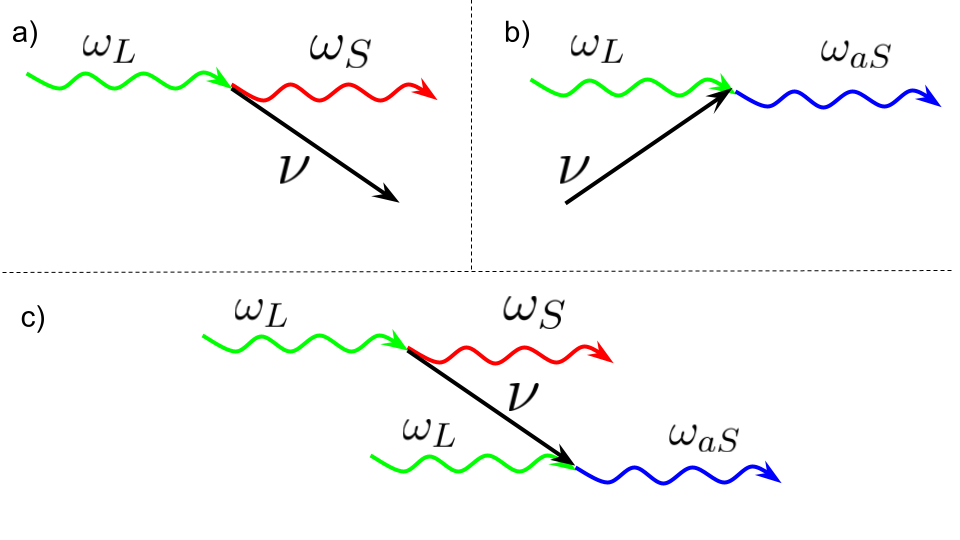
\includegraphics[scale=0.35]{Imagens_Raman.png}
\caption{Diagramas de Feynman dos processos de espalhamento Raman.  a) Stokes (S), b) anti-Stokes (aS), c) Stokes-anti-Stokes (SaS). As linhas onduladas coloridas e as setas representam fótons e fônons, respectivamente. $\omega_L$ e $\nu$ são a frequência do laser incidente e as frequências dos fônons, respectivamente, e $\omega_S$, $\omega_{aS}$ são as frequências dos campos dispersos S e aS, respectivamente.}
\label{S-aS}
\end{figure}

O principal objetivo deste projeto é aprimorar as fontes de fótons emaranhados por meio do desenvolvimento dos processos de espalhamento Raman Stokes e anti-Stokes, impulsionando o avanço de tecnologias para fontes de fótons. Para isso, serão estudadas amostras produzidas pelo laboratório com guias de onda escritas por laser de femtossegundo. Essas guias confinam a luz incidente nelas permitindo uma maior eficiencia na geração de pares de fótons S e aS. 






\section{Resultados Esperados}
Neste projeto esperamos avançar significativamente na eficiência da geração de pares de fótons correlacionados Stokes (S) e anti-Stokes (aS) por meio do efeito Raman em diamantes. Aproveitaremos estes métodos para melhor estudar as capacidades humanas de detecção da luz, especialmente de luz não clássica. Vamos desenvolver estruturas de diamante modificadas para otimizar o acoplamento fóton-fônon, aumentando a produção de pares de fótons e oferecendo insights sobre a manipulação de estados quânticos em sistemas de estado sólido.

Na comunicação quântica, a geração aprimorada de pares de fótons permitirá sistemas de repetidores quânticos mais eficientes, essenciais para a transferência de informações de longa distância com confiabilidade. Fontes de fótons de alto desempenho também apoiarão tecnologias de sensoriamento quântico, possibilitando a detecção ultraprecisa de pequenas mudanças físicas. As estruturas de diamante otimizadas desenvolvidas neste projeto podem melhorar o desempenho dos sistemas de comunicação e sensoriamento.
\section{Cronograma}
As etapas a serem realizadas, compreendem:
\begin{itemize}
   \item junho/26 - Agosto/26: Estudo teórico e leitura de bibliografia sobre efeito Raman e espalhamento Stokes-anti-Stokes.
   \item Set/26 - Dez/26: Teste de acoplamento de luz coerente nas guias de onda.
   \item Dez/26-Mar/27: Investigação experimental sobre o efeito das guias de onda na produção de pares Stokes-anti-Stokes.
   \item Mar/27-Mai/27: Obtenção e discussão dos resultados experimentais.
   \item Junho/27: Submissão de um artigo científico e divulgação do trabalho
\end{itemize}

%%%%%%%%%%%%%%%%%%%%%%%%%%% Bibliografia %%%%%%%%%%%%%%%%%%%%%%%%%%%%%%%%
\setstretch{-0.5}
\bibliographystyle{unsrt}
\bibliography{MLBR}

\end{document}